\section{Os Elementos de Euclides}
% slide 01
\begin{frame}
    \frametitle{Os Elementos de Euclides}
    \justifying
    A obra de Euclides, escrita em torno de 300 a. C é composta de 13 livros ou capítulos e reúne os conhecimentos de geometria, álgebra e aritmética. É uma obra que foi amplamente divulgada, sendo o livro mais editado após a Bíblia. 
    \vspace{3mm}

    Reunindo o conhecimento das matemáticas de seu tempo e, embora algumas demonstrações sejam de autoria de Euclides, sua maior contribuição está na apresentação axiomática desse conhecimento.

    \begin{figure}[H]
        \centering
        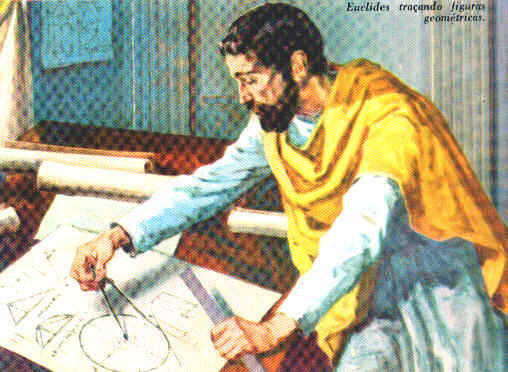
\includegraphics[scale=0.30]{img/elements.jpg}
    \end{figure}
\end{frame}

\section{Os Treze Livros}
% slide 02
\begin{frame}
    \frametitle{Os Treze Livros}
    \begin{itemize}
        \item Os livros I-IV tratam de \textbf{geometria plana elementar}
        \item O livro V apresenta a \text{teoria das proporções de Eudoxo} na sua forma puramente geométrica
        \item O livro VI aplica-a semelhança de \textbf{figuras planas}
        \item Os livros VII-IX são dedicados à \textbf{teoria dos números}
        \item O livro X, os mais extenso de todos e muitas vezes considerado o mais difícil, contém a classificação geométrica de \textbf{irracionais quadráticos} e as suas raízes quadráticas
        \item O livros XI-XIII ocupam-se com a \textbf{geometria sólida}
    \end{itemize}
\end{frame}

\section{Livros I-IV}
% slide 03
\begin{frame}
    \frametitle{Livros I-IV}
    \justifying
    Conforme dito no slide anterior, os livros de I-IV tratam de geometria plana, partindo das mais elementares propriedades de rectas e ângulos conduzem à congruência de triângulos, à igualdade de áreas, ao teorema de Pitágoras.
    \vspace{3mm}
    
    Como a maioria dos treze livros, o livro I começa com uma lista de Definições (23, ao todo) sem qualquer comentário como, por exemplo, as de ponto, reta, círculo, triângulo, ângulo, paralelismo e perpendicularidade de retas tais como:
    \vspace{3mm}
    \begin{itemize}
        \item Ponto é o, que não tem partes, ou o, que não tem grandeza alguma.
        \item Linha é o, que tem comprimento sem largura.
        \item As extremidades da linha são pontos.
        \item Linha reta é aquela, que está posta igualmente entre as suas extremidades.
    \end{itemize}
\end{frame}

% slide 04
\begin{frame}
    \frametitle{Livros I-IV}
    \justifying
    Após as definições, aparecem os Postulados e as Noções Comuns ou Axíomas. Os Postulados são proposições geométricas específicas. \textit{"Postular"} significa \textit{"pedir para aceitar"}. Assim, Euclides pede ao leitor para aceitar as cinco proposições geométricas que formula nos Postulados:
    \vspace{3mm}
    
    \begin{enumerate}
        \item Pode-se traçar uma (única) reta ligando quaisquer dois pontos.
        \item Pode-se continuar (de uma única maneira) qualquer reta finita continuamente em uma reta.
        \item Pode-se traçar um círculo com qualquer centro e com qualquer raio.
        \item Todos os ângulos retos são iguais.
        \item Sejam duas retas $m$ e $n$ cortadas por uma terceira reta $r$. Se a soma dos ângulos formados é menor do que 180 graus, então $m$ e $n$ não são paralelas. Além disso, elas se intersectam do lado dos ângulos cuja soma é menor do que 180 graus.
    \end{enumerate}
\end{frame}

\section{O Quinto Postulado de Euclides}
% slide 05
\begin{frame}
    \frametitle{O Quinto Postulado de Euclides}

    \textbf{Proposição 28:} \textit{Sejam duas retas m e n cortadas por uma terceira reta r. Se a soma dos ângulos formados (ver figura 1.2) é 180 graus, então m e n são retas paralelas.}

    \begin{equation}
        \alpha + \beta = 180^o \Rightarrow m \cap n = \emptyset
    \end{equation}

    \begin{figure}[h!]
        \centering
        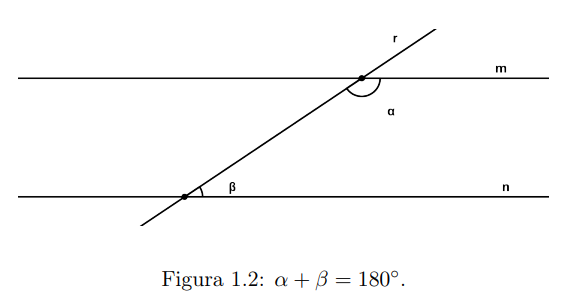
\includegraphics[scale=0.55]{img/retas_paralelas.png}
    \end{figure}
\end{frame}

% slide 06
\begin{frame}
    \frametitle{O Quinto Postulado de Euclides}
    \justifying
    E a recíproca, é verdadeira? Ou seja, é verdade que

    \begin{equation}
        m \cap n = \emptyset \Rightarrow \alpha + \beta = 180^o
    \end{equation}

    A resposta a essa pergunta é complexa e levou mais de dois mil anos para ser entendida completamente. De fato, esta recíproca é exatamente o conteúdo do Postulado 5.

\end{frame}

% slide 07
\begin{frame}
    \frametitle{O Quinto Postulado de Euclides}
    \justifying
    \textbf{Postulado 5.} \textit{Sejam duas retas m e n cortadas por uma terceira reta r. Se a soma dos ângulos formados (ver figura) é menor do que 180 graus, então m e n não são paralelas. Além disso, elas se intersectam do lado dos ângulos cuja soma é menor do que 180 graus.}

    \begin{figure}[h!]
        \centering
        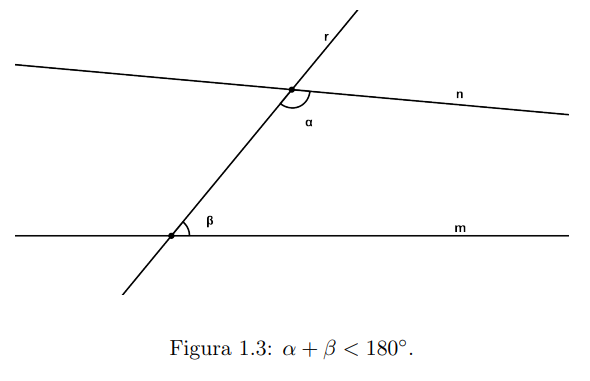
\includegraphics[scale=0.55]{img/postulado5.png}
    \end{figure}

\end{frame}

\section{Considerações Finais}
% slide 08
\begin{frame}
    \frametitle{Considerações Finais}
    \justifying

    \begin{figure}[!h]
        \centering
        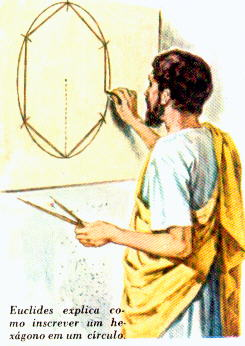
\includegraphics[scale=0.35]{img/euclid2.jpg}
    \end{figure}

    \hspace{5mm}Euclides compilou nos Elementos toda a geometria conhecida na sua época. Mas, não se limitou a reunir todo o conhecimento geométrico, ordenou-o e estruturou-o como ciência. Isto é, a partir de uns axiomas desenvolveu e demonstrou os teoremas e proposições geométricas, dando novas demonstrações quando as antigas não se adaptavam à nova ordem que havia dado às proposições. Além disso, esmiuçou a fundo as propriedades das figuras geométricas, das áreas e dos volumes e estabeleceu o conceito de lugar geométrico.
\end{frame}